\subsection{Introduction}

% \begin{itemize}
%     \item Similar introduction to the COG paper updated with the research papers that have come out since then (and others) \citepsixth{p6Cook2016-SecondPaperDanesh,Khalifa2019-intentionalCompLevel,gravina2019procedural,Gravina2019-blendingNotionsDiversity,fontaine2019covariance,ashlock2019-dowhatspossible,machado2019evaluation} and a bit more focus on the evaluation of PCG tools.
% \end{itemize}{}

Procedural Content Generation (PCG) refers to the generation of game content with none or limited human input~\citepsixth{p6Yannakakis2018}, where game content could be anything from rules and narrative, to levels, items, and music. While PCG has been a factor in game development since trailblazing games like~\emph{Rogue}~\citepsixth{p6michael_toy_1980} and \emph{Elite}~\citepsixth{p6braben_elite_1984}, it has only been a popular academic research topic for little more than a decade. Search-based PCG designates the use of a global search algorithm, such as an evolutionary algorithm to search content space~\citepsixth{p6Togelius2011}.

% Allure is in this context mainly negating the work done by the referenced material. cf. Lure
Part of PCG's appeal is the promise to produce game art and content faster and at a lower cost, as well as enabling innovative content creation processes such as player-adaptive games~\citepsixth{p6shaker2012evolving,p6hastings_evolving_2009,p6dormansUnexplored2017}, data-driven content generation~\citepsixth{p6Khalifa2018,p6Green2018}, and mixed-initiative co-creativity~\citepsixth{p6Liapis2016}. Mixed-initiative co-creativity (MI-CC), a concept introduced by Yannakakis et al.~\citepsixth{p6yannakakis2014micc}, refers to the approach of using a creation process through which a computer and a human user provide %feed
and inspire each other in the form of iterative reciprocal stimuli. Examples of MI-CC systems are \textit{Pitako}~\citepsixth{p6machado2019pitako}, \textit{Ropossum}~\citepsixth{p6shaker2013ropossum}, \textit{Tanagra}~\citepsixth{p6smith_tanagra:_2011}, \textit{CICERO}~\citepsixth{p6Machado2017}, and \textit{Sentient Sketchbook}~\citepsixth{p6liapis_generating_2013}. 

MI-CC aligns with the principles of lateral thinking and creative emotive reasoning: the processes of solving seemingly unsolvable problems or tackling non-trivial tasks through an indirect, non-linear, creative approach~\citepsixth{p6Liapis2016}. Additionally, MI-CC provides insight on the affordances and constraints of the human process for creating and designing games~\citepsixth{p6Yannakakis2018}.

A key mechanism in MI-CC approaches is to present suggestions to users%players
, and these suggestions must be of high quality but also be sufficiently diverse. So-called quality-diversity algorithms~\citepsixth{p6Pugh2016} are very well suited for this, as they find solutions that have high quality according to some measure but are also diverse according to other measures~\citepsixth{p6gravina2019procedural}. The Multi-dimensional Archive of Phenotypic Elites (MAP-Elites)~\citepsixth{p6Mouret2015} is a suitable algorithm for this kind of problem. Khalifa et al.~\citepsixth{p6Khalifa2018} presented constrained MAP-Elites, a combination MAP-Elites with the feasible-infeasible concept from the FI2Pop genetic algorithm~\citepsixth{p6Kimbrough2008}, and applied this to procedurally generating levels for bullet hell games. %Another implementation of MAP-Elites has been recently used to produce small sections of Super Mario Bros levels called \textit{scenes}, addressing specific game mechanics \citepsixth{p6Khalifa2019-intentionalCompLevel}.
Another recent implementation of MAP-Elites has been used to produce small sections of Super Mario Bros levels called \textit{scenes}, addressing specific game mechanics~\citepsixth{p6Khalifa2019-intentionalCompLevel}.

The Evolutionary Dungeon Designer (EDD) is a MI-CC tool for generating dungeons for adventure games using a FI2Pop evolutionary approach~\citepsixth{p6Alvarez2018,p6Alvarez2018a,p6Baldwin2017,p6Baldwin2017a}. This %paper extends the previous
research was presented in~\citepsixth{p6alvarez2019empowering}, %which introduced 
introducing \emph{Interactive Constrained MAP-Elites} (IC MAP-Elites), a combination of Constrained MAP-Elites with interactive evolution, in the shape of %EDD's FI2Pop evolutionary algorithm,
%The algorithm was implemented as 
a continuous evolutionary process that takes advantage of MAP-Elites' multidimensional discretization of the search space into cells. %The previous paper
In \citepsixth{p6alvarez2019empowering}, we analyzed the effects of using quality-diversity in procedurally generating dungeons, as well as the effects of continuous evolution and dimension customization.% in a MI-CC approach. %In the current work, 

This paper contributes with %we conduct an in-depth analysis of the behaviour of the algorithm 
a thorough evaluation of the expressive range of EDD's MAP-Elites through all possible dimension combinations in several scenarios, as well as by extending the feature dimensions to %include 
two new dimensions, \emph{Inner similarity}, which adds a similarity measure independent of the aesthetics, and \emph{Leniency}, which strives to measure the subjective challenge score of a level. Following recent research on how to evaluate procedural content generators and, in particular, quality-diversity approaches~\citepsixth{p6Cook2019:ParameterBasedEvaluation,p6Cook2016-SecondPaperDanesh,p6Gravina2019-blendingNotionsDiversity}, we present the results from new experiments %run 
with the objective to evaluate the expressive range of all dimensions in pairs, as well as to analyze how the generated and unique solutions relate to all the dimensions included in the search space, and assess IC MAP-Elites feasibility and adaptability to create dungeons and adventure levels.

% \begin{figure}[t]
% \centerline{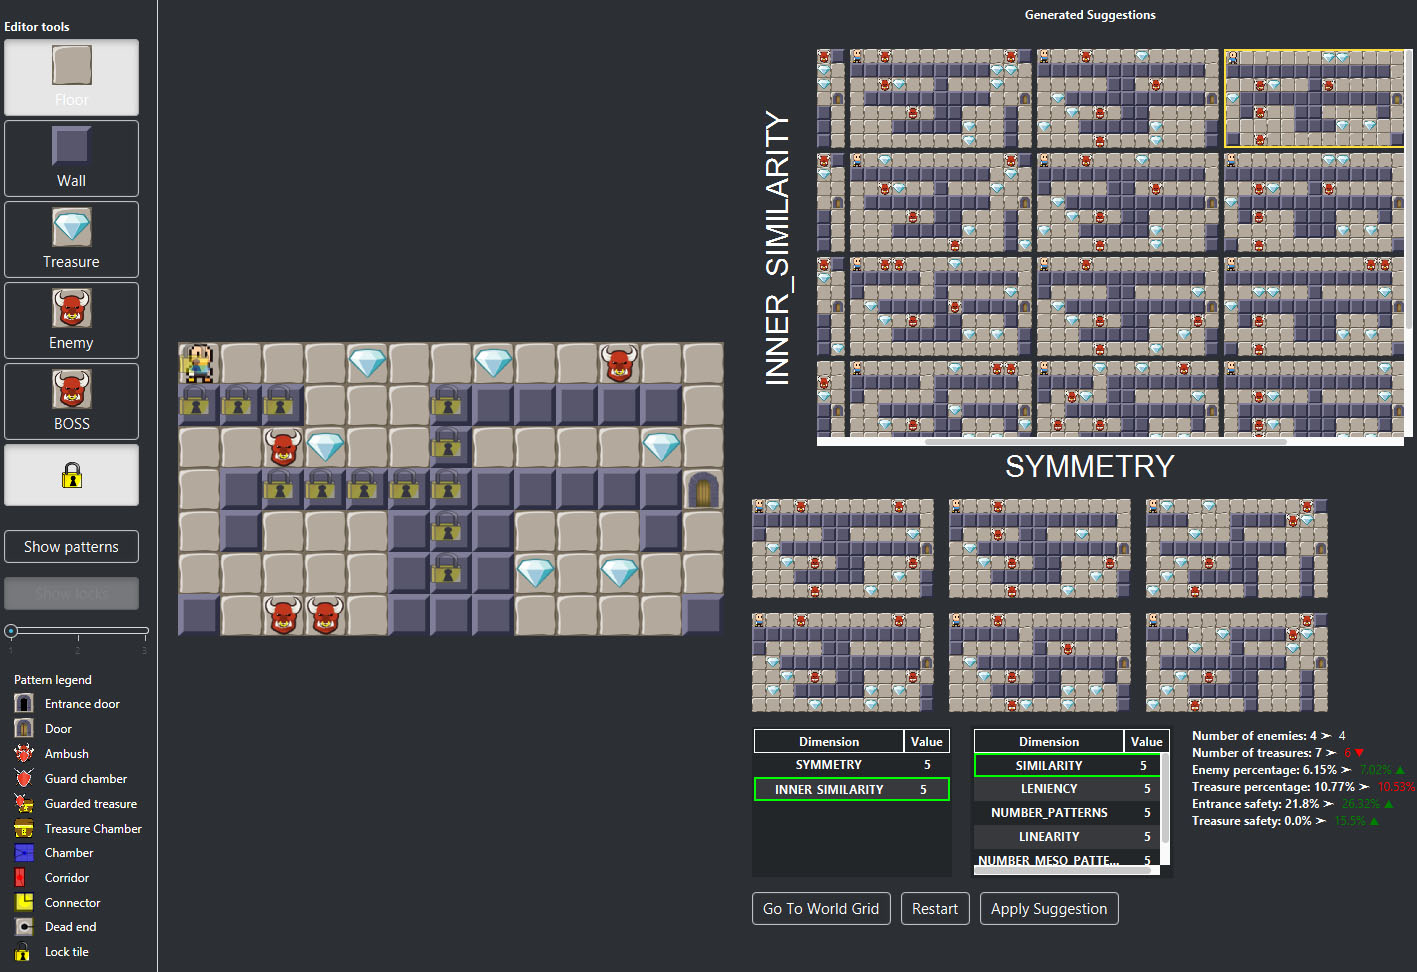
\includegraphics[width=9cm]{figures/figure1.png}}
% \caption{The main components in EDD. (a) A basic room, (b) different placeable tiles, (c) micro-patterns and (d) meso-patterns~\citepsixth{p6Alvarez2018a}.}
% \label{figs:basecomponents}
% \end{figure}